\chapter{Electrical Characterisation and Analysis}

This chapter presents the electrical characterisation and critical analysis
of the depletion-mode GaAs/AlGaAs HEMT devices fabricated using the unrecessed
process described in Chapter~3. The measurements reported here are intended
to establish a robust baseline against which subsequent enhancement-mode devices may be evaluated next semester.

Characterisation was performed across the full array of fifteen devices,
comprising five gate lengths with three nominally identical repeats of each
geometry. The analysis therefore focuses not only on individual device
performance, but also on geometry-dependent trends and device-to-device
variability arising from fabrication and electrostatic effects.

\section{Measurement Setup}

Electrical measurements were carried out using a Keysight B1500A
semiconductor device parameter analyser \cite{leedscleanroom_equipment} under ambient laboratory conditions
at room temperature (\SI{21}{\degree C}).

Output characteristics were obtained by sweeping the drain--source voltage
($V_{DS}$) at fixed gate voltages in order to examine linear-region conduction
and current saturation behaviour. Transfer characteristics were measured by
sweeping the gate--source voltage ($V_G$) at a fixed drain bias chosen to
ensure operation within the saturation regime. From these measurements, the
drain current ($I_D$), transconductance ($g_m$), and threshold behaviour were
extracted.

Channel resistance was determined from the low-bias linear region of the
output characteristics, where the device operates in the ohmic regime. A
consistent drain--source voltage range was used for all devices to enable
direct comparison between gate geometries. Transconductance was calculated
numerically from the measured $I_D$--$V_G$ data using finite-difference methods,
with identical differentiation procedures applied throughout.

For each gate geometry, electrical characteristics were averaged across three
nominally identical devices to provide a representative response while
suppressing random device-to-device variation.

\section{Output Characteristics}

The output characteristics of the fabricated depletion-mode HEMTs were measured
to assess channel conduction, current saturation behaviour, and gate-length
scaling within the unrecessed process. Figure~\ref{fig:id-vds} shows the
measured $I_D$--$V_{DS}$ characteristics, presented both as averaged responses
for each gate geometry and as a direct comparison between the shortest and
longest gate-length devices.

\begin{figure}[htbp]
  \centering
  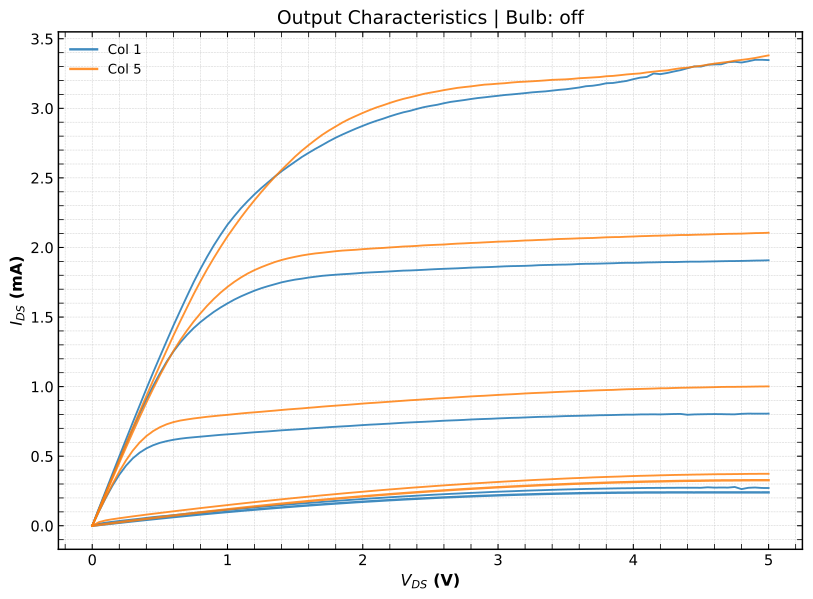
\includegraphics[width=0.75\linewidth]{figures/electrical_analysis/col1_vs_col5_ID.png}
  \caption{Measured output characteristics ($I_D$--$V_{DS}$) of the fabricated
    depletion-mode GaAs/AlGaAs HEMTs. Curves show averaged responses for each
    gate length, with comparison between the shortest (Orange) and longest (Blue) gate
    geometries highlighted.}
  \label{fig:id-vds}
\end{figure}

Across all gate geometries, the devices exhibit a clear linear region at low
drain--source voltage followed by well-defined current saturation at higher
$V_{DS}$. The linear-region behaviour confirms low-resistance ohmic contacts
and uniform channel formation across the device array. The onset of saturation
is consistent with electrostatic pinch-off near the drain, indicating effective
gate control of the channel.

A systematic dependence of drain current on gate length is observed. Devices
with shorter gate lengths exhibit increased drain current at a given gate
bias, consistent with reduced channel resistance and enhanced current drive.
This trend is monotonic across the full set of geometries and is preserved in
the averaged characteristics, indicating that it reflects intrinsic
gate-length scaling rather than random device-to-device variation.

Importantly, no significant degradation in saturation behaviour is observed
for the shortest gate devices within the measured bias range. The saturation
regions remain relatively flat across all geometries, suggesting that
short-channel effects such as drain-induced barrier lowering are not dominant
for the gate lengths investigated. This supports the validity of treating
these devices as long-channel references for subsequent electrostatic and
threshold-voltage analysis.

Comparison between the three nominally identical devices for each gate geometry
reveals a high degree of repeatability in the output characteristics. The close
overlap of curves within each geometry indicates that process-induced
variability, including contact resistance fluctuations and local
heterostructure non-uniformity, is small relative to the systematic trends
introduced by gate-length variation.

Overall, the output characteristics demonstrate predictable scaling with gate
length, robust current saturation, and good repeatability across the device
array. These results confirm the electrical integrity of the baseline
depletion-mode fabrication process and establish a reliable reference against
which the impact of gate recession and enhancement-mode operation can be
assessed in later stages of this project.

\section{Transfer Characteristics}

The gate transfer characteristics were measured to evaluate electrostatic
control of the channel, threshold behaviour, and the influence of gate length
on current modulation in the unrecessed depletion-mode devices.
Figure~\ref{fig:id_vg} presents the measured $I_D$--$V_G$ characteristics,
shown as averaged responses for each gate geometry together with a direct
comparison between the shortest and longest gate-length devices.

\begin{figure}[h]
    \centering
    
\includegraphics[width=0.9\linewidth]{figures/electrical_analysis/gate_transfer.png}
    \caption{Measured transfer characteristics ($I_D$--$V_G$) of the fabricated
    depletion-mode GaAs/AlGaAs HEMTs. Curves show averaged responses for each
    gate length, with comparison between the shortest and longest gate
    geometries highlighted.}
    \label{fig:id_vg}
\end{figure}

All devices exhibit clear depletion-mode behaviour, with substantial drain
current present at zero gate bias and progressive channel pinch-off as the
gate voltage is made more negative. The smooth and monotonic dependence of
$I_D$ on $V_G$ across all geometries indicates effective gate control of the
two-dimensional electron gas and an absence of significant trapping or
hysteresis effects within the measured bias range.

The extracted threshold voltage is broadly consistent across gate lengths,
with only modest variation observed between geometries. This behaviour is
expected for long-channel, unrecessed HEMTs in which the threshold voltage is
primarily set by the vertical electrostatics of the heterostructure rather
than lateral device dimensions. The weak dependence of threshold voltage on
gate length therefore supports the assumption that short-channel effects are
minimal in the present device set.

At a given gate overdrive, devices with shorter gate lengths exhibit higher
drain current, reflecting reduced channel resistance and increased current
drive. This trend is consistent with the scaling observed in the output
characteristics and confirms that lateral gate-length variation primarily
modulates channel conductance rather than the onset of channel formation. The
similarity of the subthreshold-to-on transition across geometries further
indicates that the electrostatic coupling between the gate and the channel is
not significantly degraded for shorter gate lengths within the range
investigated.

Repeatability across the three nominally identical devices for each geometry
is high, with close overlap observed in the averaged transfer characteristics.
The limited spread in both threshold voltage and slope suggests that
fabrication-induced variability, such as fluctuations in donor density or
Schottky barrier quality, is small relative to the systematic effects of gate
length scaling. This level of uniformity is particularly important in the
context of subsequent gate recessing, where small variations in vertical
geometry are expected to produce comparatively large shifts in threshold
voltage.

Overall, the transfer characteristics confirm strong and consistent gate
control of the channel, stable depletion-mode operation, and weak
gate-length dependence of threshold voltage. These results validate the use of
the present device set as a reliable electrical baseline for assessing the
impact of controlled gate recession in enhancement-mode devices fabricated in
the second phase of this project.

\section{Gate Leakage Behaviour}

\section{Threshold-Voltage Extraction}

\section{Variability, Non-Idealities and Interpretation}

\section{Implications for Process Control and Device Behaviour}
